% sgn sin(nx) for n = 2 and n = 12. Generated by a short script.
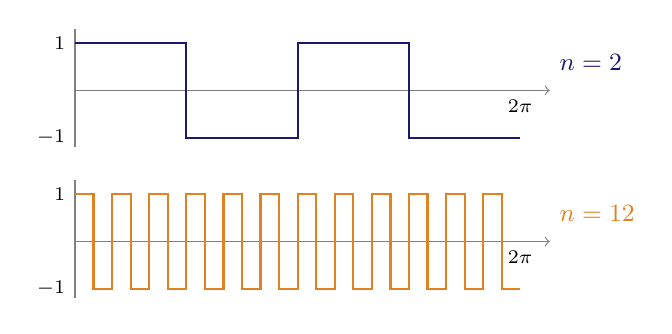
\begin{tikzpicture}[xscale=0.9,yscale=0.6]
\draw[->,black!50] (0,0) -- (6.7,0);
\draw[black!50] (0,-1.2) -- (0,1.3);
\draw[MidnightBlue,thick] (0.0000,1.0000) -- (1.5708,1.0000) -- (1.5708,-1.0000) -- (3.1416,-1.0000) -- (3.1416,1.0000) -- (4.7124,1.0000) -- (4.7124,-1.0000) -- (6.2832,-1.0000);
\node[left,font=\scriptsize] at (0,1) {$1$};
\node[left,font=\scriptsize] at (0,-1) {$-1$};
\node[below,font=\scriptsize] at (6.2832,0) {$2\pi$};
\node[right,font=\small,MidnightBlue] at (6.7,0.6) {$n=2$};
\draw[->,black!50] (0,-3.2) -- (6.7,-3.2);
\draw[black!50] (0,-4.4) -- (0,-1.9000000000000001);
\draw[BurntOrange!90!black,thick] (0.0000,-2.2000) -- (0.2618,-2.2000) -- (0.2618,-4.2000) -- (0.5236,-4.2000) -- (0.5236,-2.2000) -- (0.7854,-2.2000) -- (0.7854,-4.2000) -- (1.0472,-4.2000) -- (1.0472,-2.2000) -- (1.3090,-2.2000) -- (1.3090,-4.2000) -- (1.5708,-4.2000) -- (1.5708,-2.2000) -- (1.8326,-2.2000) -- (1.8326,-4.2000) -- (2.0944,-4.2000) -- (2.0944,-2.2000) -- (2.3562,-2.2000) -- (2.3562,-4.2000) -- (2.6180,-4.2000) -- (2.6180,-2.2000) -- (2.8798,-2.2000) -- (2.8798,-4.2000) -- (3.1416,-4.2000) -- (3.1416,-2.2000) -- (3.4034,-2.2000) -- (3.4034,-4.2000) -- (3.6652,-4.2000) -- (3.6652,-2.2000) -- (3.9270,-2.2000) -- (3.9270,-4.2000) -- (4.1888,-4.2000) -- (4.1888,-2.2000) -- (4.4506,-2.2000) -- (4.4506,-4.2000) -- (4.7124,-4.2000) -- (4.7124,-2.2000) -- (4.9742,-2.2000) -- (4.9742,-4.2000) -- (5.2360,-4.2000) -- (5.2360,-2.2000) -- (5.4978,-2.2000) -- (5.4978,-4.2000) -- (5.7596,-4.2000) -- (5.7596,-2.2000) -- (6.0214,-2.2000) -- (6.0214,-4.2000) -- (6.2832,-4.2000);
\node[left,font=\scriptsize] at (0,-2.2) {$1$};
\node[left,font=\scriptsize] at (0,-4.2) {$-1$};
\node[below,font=\scriptsize] at (6.2832,-3.2) {$2\pi$};
\node[right,font=\small,BurntOrange!90!black] at (6.7,-2.6) {$n=12$};
\end{tikzpicture}
